\chapter{The Magnetic Field}

\section{Introduction}

In this lab, we will determine the strength of the magnetic field in the gap of an electromagnet in two ways: first, by measuring the force applied on a current-carrying rod; and second, by measuring the effects of changing magnetic flux through a coil that is being inserted or removed from that gap. In doing so, we will also be verifying both Faraday's law and Lenz's law! \myskip

\underline{\textbf{CAUTION:}}
\begin{itemize}
 \item Always reduce the current through the electromagnet to zero before opening the circuit of the magnet coils.
 \item Remove wrist watches before placing hands near the magnet gaps.
\end{itemize}

\section{Theory}
\subsection{Force on a Current-carrying Wire}
Consider a rod of length $L$, held horizontally and normal to the direction of a uniform, horizontal magnetic field $B$. If a current $i$ is passed through the wire, as indicated in Figure {\ref{fig:force}}, then there will be a vertical force $F=iLB$ on the wire rod.
\begin{figure}[h]
\centering
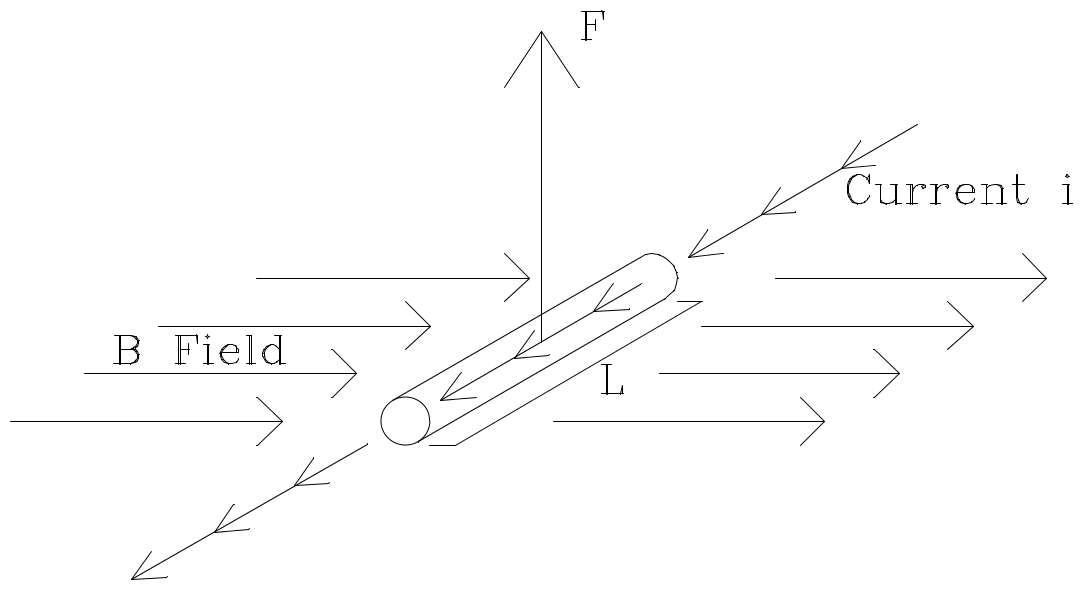
\includegraphics[width=0.6\textwidth]{./Exp4/pic/image1.png}
\caption{Force on a Current-carrying Wire}
\label{fig:force}
\end{figure}

\subsection{Induced EMF in a Coil}
According to Faraday's Law of induction, a changing magnetic flux through a coil induces an EMF (electromagnetic force) $\varepsilon$ given by
\begin{equation}
 \varepsilon=N\frac{\Delta \Phi}{\Delta t}
\end{equation}
where $\Phi = \int \vec{B} \cdot d \vec{A}$ is the flux of magnetic field $B$ through a coil of area $A$ and perpendicular to that area. $N$ is the number of turns in the search coil. For this experiment, the area of the coil is constant and the magnetic field is assumed to be uniform, so the average EMF is given by
\begin{equation}
 \varepsilon= -NA\frac{\Delta B}{\Delta t}
 \label{eq:emf}
\end{equation}
The negative sign in Faraday's Law comes from the fact that the EMF induced in the coil acts to oppose any change in the magnetic field. This is summarized as Lenz' Law. It is important to remember that EMF, despite being called a "force" is actually a potential and is measured in volts. Voltage will be induced as the coil enters and leaves magnetic field and its direction will be determined using Lenz' law.

\section{Procedure}
\subsection{Force on a Current-carrying Wire}

The experimental set-up is shown in Figure {\ref{fig:set-up}}. The horizontal magnetic field $B$ is produced in the air gap of a ``C-shaped'' iron electromagnet. The strength of $B$ is determined by the current in the magnet coils $I$, which is supplied by an adjustable low-voltage power supply.\myskip
\begin{figure}[h]
\centering
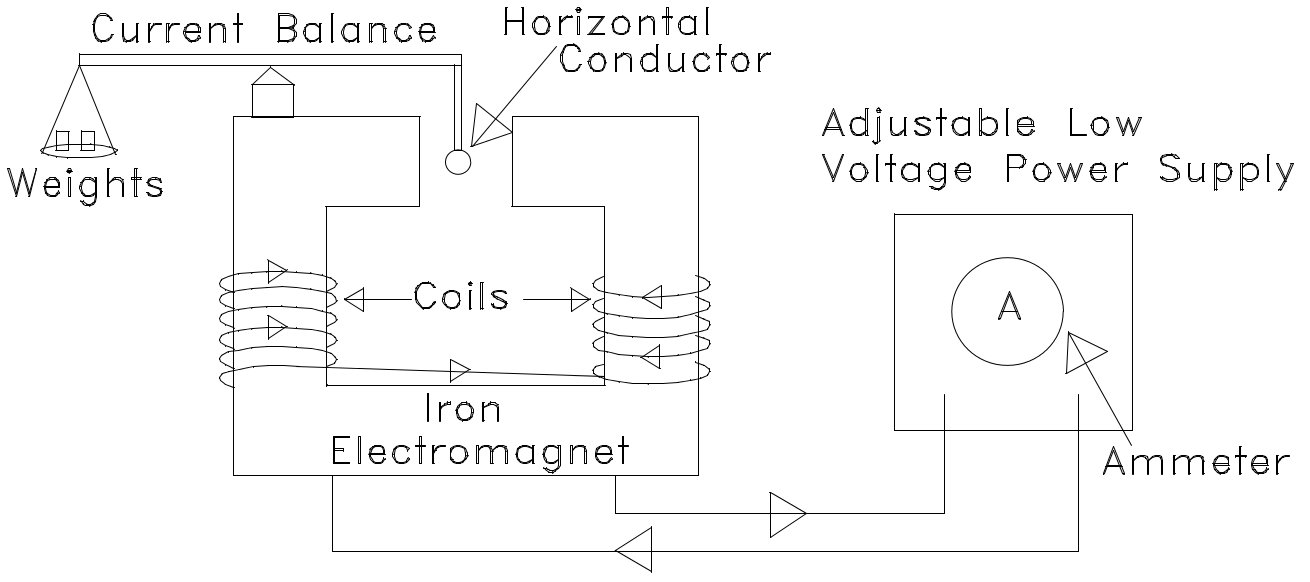
\includegraphics[width=0.8\textwidth]{./Exp4/pic/image2.png}
\caption{Experimental Set-up}
\label{fig:set-up}
\end{figure}

A more detailed drawing of the balance and electromagnet arrangement is shown in Figure {\ref{fig:measureforce}}.

\begin{figure}[h]
\centering
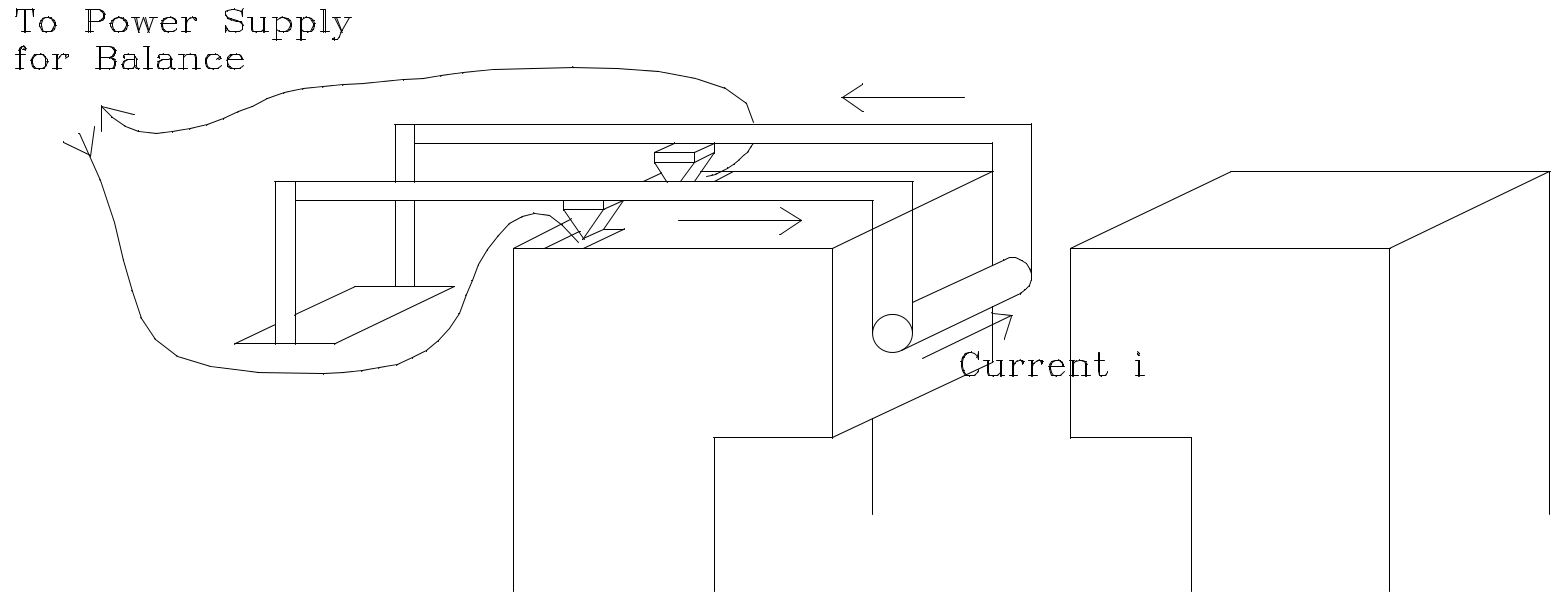
\includegraphics[width=0.8\textwidth]{./Exp4/pic/image3.png}
\caption{Setup of the Wire and Balance for Force Measurement}
\label{fig:measureforce}
\end{figure}

Note that the current $i$ through the horizontal conductor is supplied by a separate power supply. The current balance is constructed out of conducting and insulating materials such that current can enter through one side of the knife-edge fulcrum, flow through one side of the balance arm to the horizontal conductor, and then flow back through the other side of the balance arm and out through the other knife-edge. \myskip

The current $i$ in the balance is provided by the HP E3610A power supply, which can operate either in constant voltage or constant current mode. The voltage dial sets the \emph{maximum voltage} the device will supply to the circuit; the current dial likewise sets the \emph{maximum current}, and if the circuit tries to draw more current, the power supply will reduce the voltage until it reaches whatever value is needed to maintain the maximum current (by $V = IR$). \myskip

To use the power supply in constant current mode, begin with the current dial turned all the way down (counter-clockwise) and the voltage dial turned all the way up (clockwise). Set the range to 3 Amps, and connect the leads to the $+$ and $-$ terminals. You can now set the current to the desired level. Note that the digital meters on the power supply show the \emph{actual} voltage and current being supplied, so you will not normally see any current unless the leads are connected to a complete circuit. (If you want to set the current level without closing the circuit, you can hold in the CC Set button while you turn the current dial.) Once you close the circuit, the voltage adjusts automatically to maintain the constant current level, and the CC (Constant Current) indicator light should be on.

\begin{enumerate}
 \item Set the current $I$ through the electromagnet at 5 amperes. Place a small number of weights on the balance and determine the value off $i$ necessary to reach equilibrium. Repeat for at least five different weights.

 \item With Microsoft Excel, plot the weight used to balance the scale vs. the balance current $i$. Include error bars.

 \item Draw a line of best fit and determine the slope with error using LINEST.

 \item From your slope, determine the magnetic field strength $B$ with error.

 \item Repeat the above steps (steps 1-4) for two other magnet currents $I$ (for a total of three current data sets). You do not need to do error analysis for these measurements, but plot each of your results on the same graph.

 \item Draw a diagram similar to Figure \ref{fig:measureforce} and indicate the directions of $i$, $F$ and $B$ for your setup.

 \item Discuss potential sources of error.
\end{enumerate}

\subsection{Induced EMF in a Coil}

\begin{figure}[h]
\centering
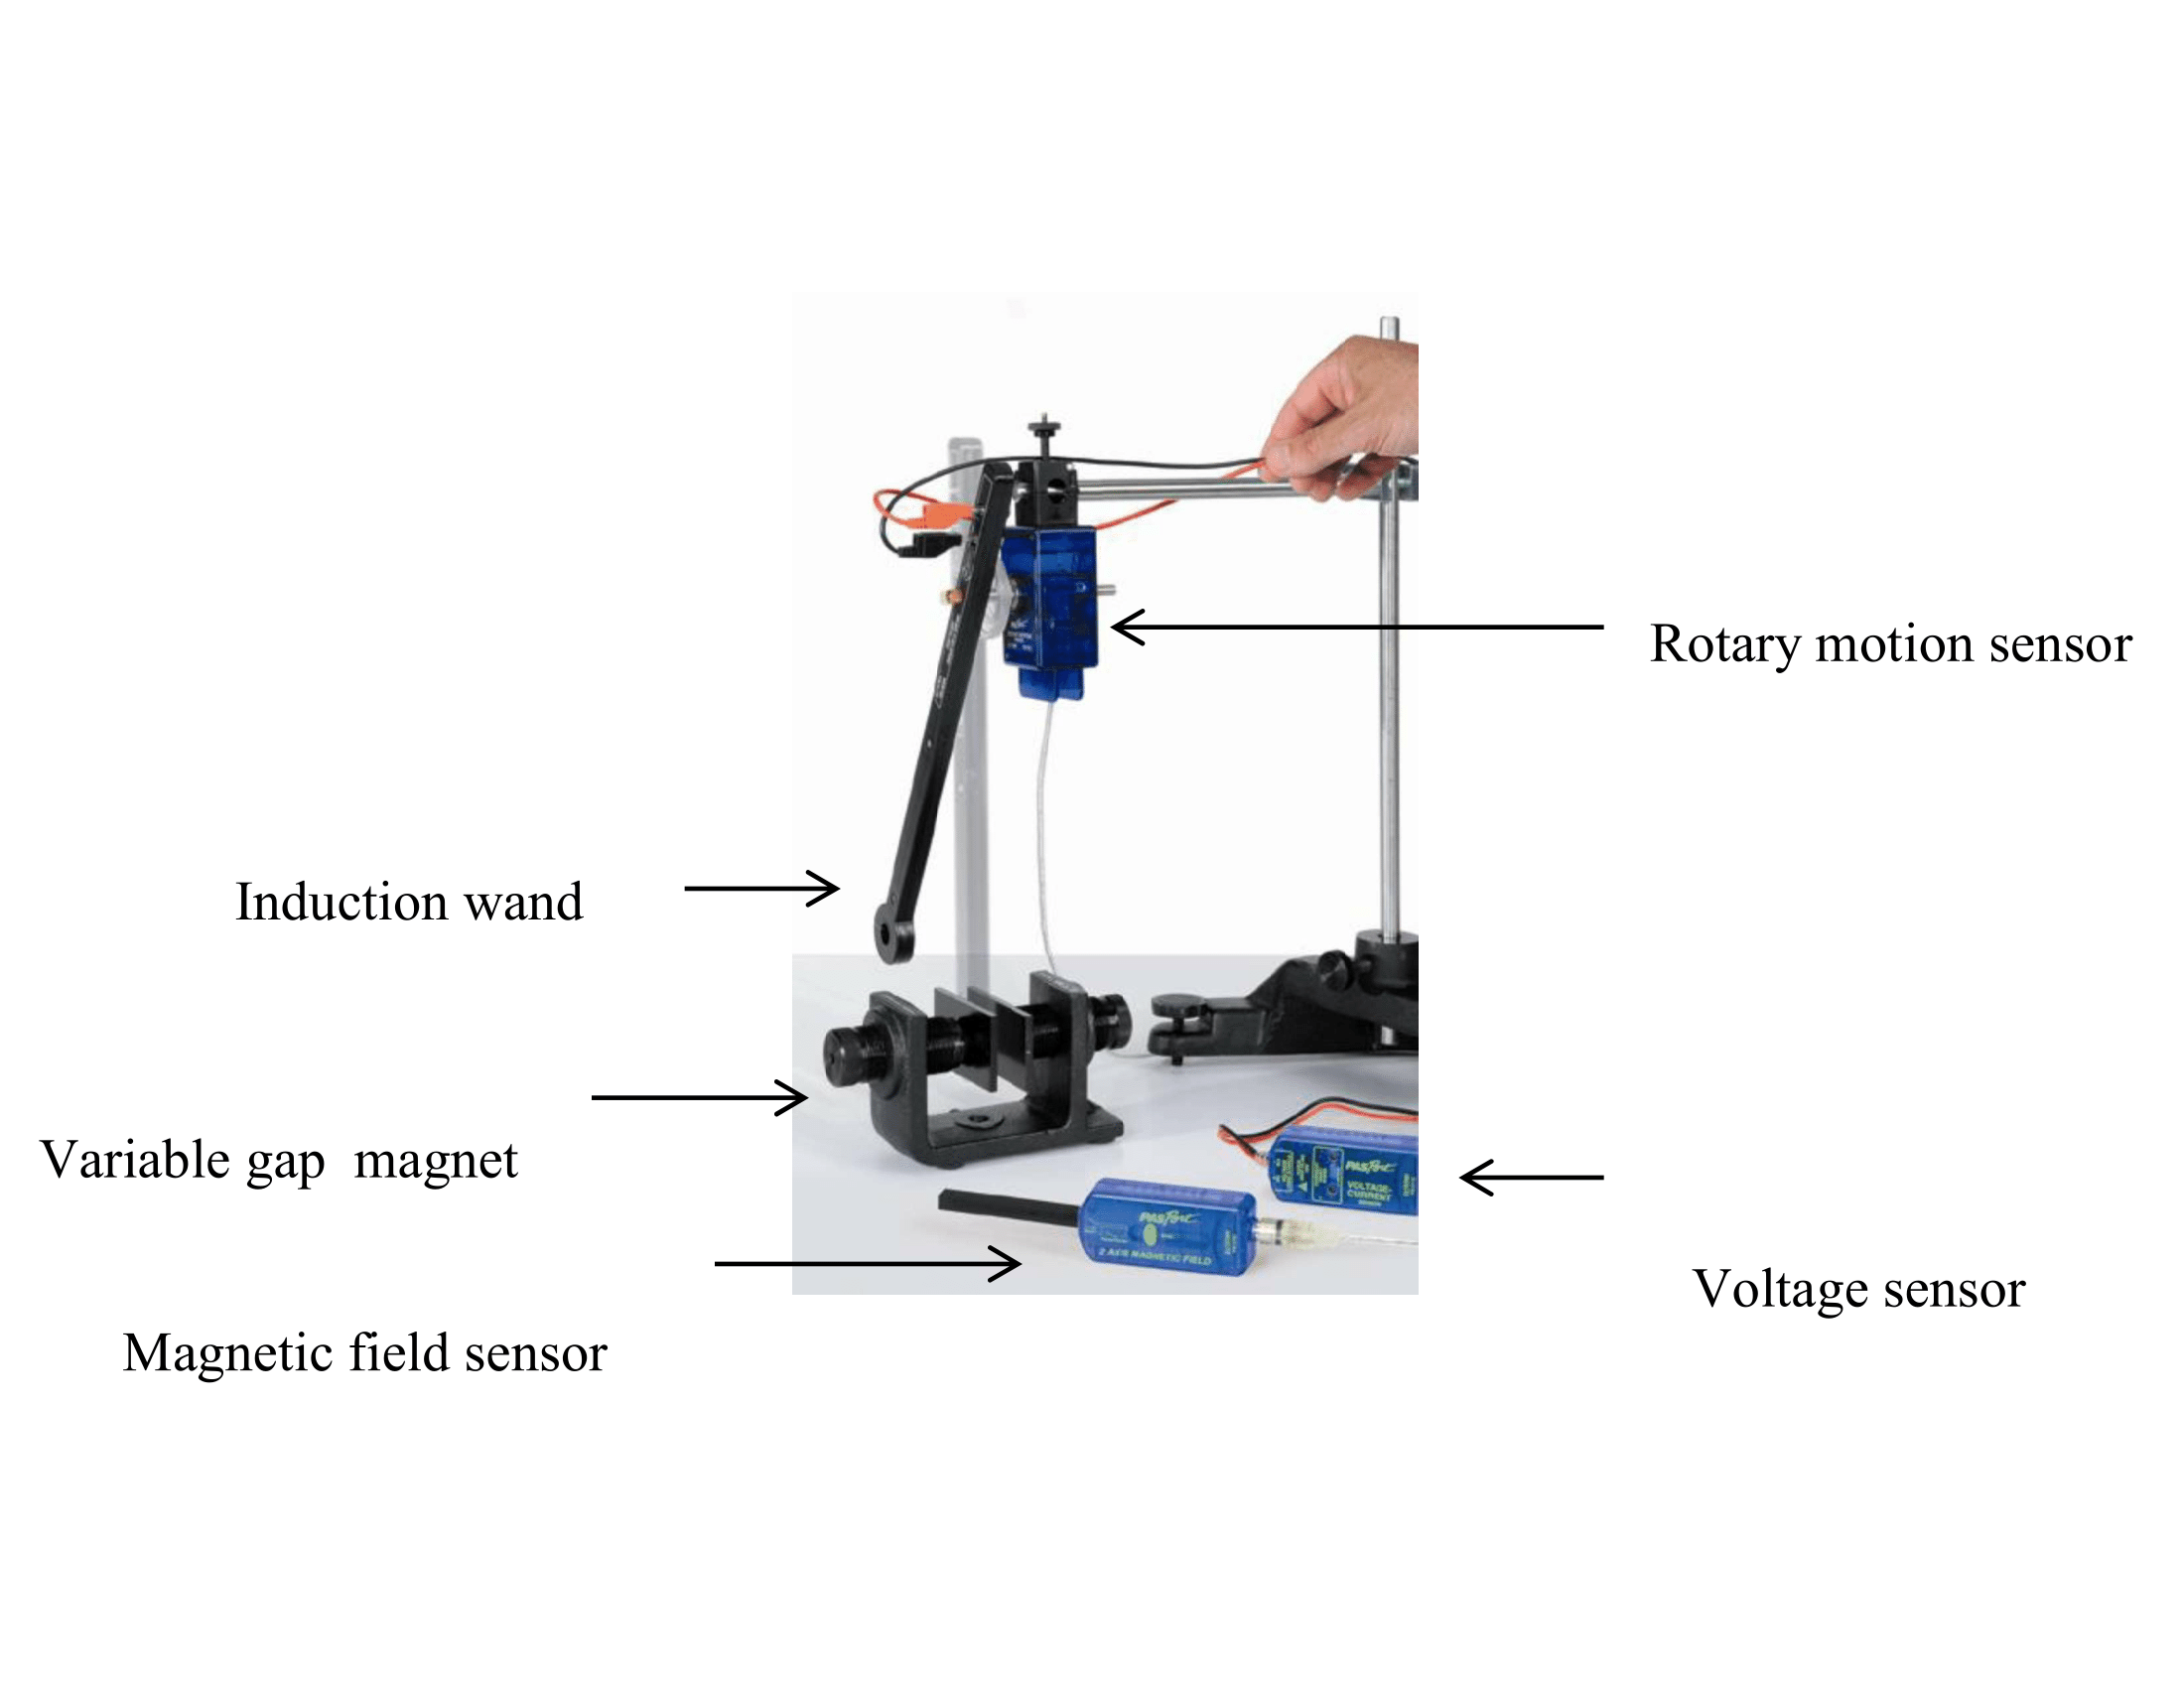
\includegraphics[width=0.85\textwidth]{./Exp4/pic/emf_setup.png}
\caption{Apparatus of the magnetic field sensor}
\label{fig:emfsetup}
\end{figure}

Figure \ref{fig:emfsetup} shows the initial setup for this experiment. A rotary motion sensor is attached to the end of the cross-rod. It also acts as a pivot for the induction wand. The induction wand is a rigid pendulum with a coil at its end that will swing through a variable gap magnet. The coil in the induction wand comprises 200 turns with an outer diameter of 3.1 cm. When the coil passes the gap in between the magnet, it experiences a change in magnetic field and EMF is induced in the coil.\myskip

\begin{figure}[h]
\centering
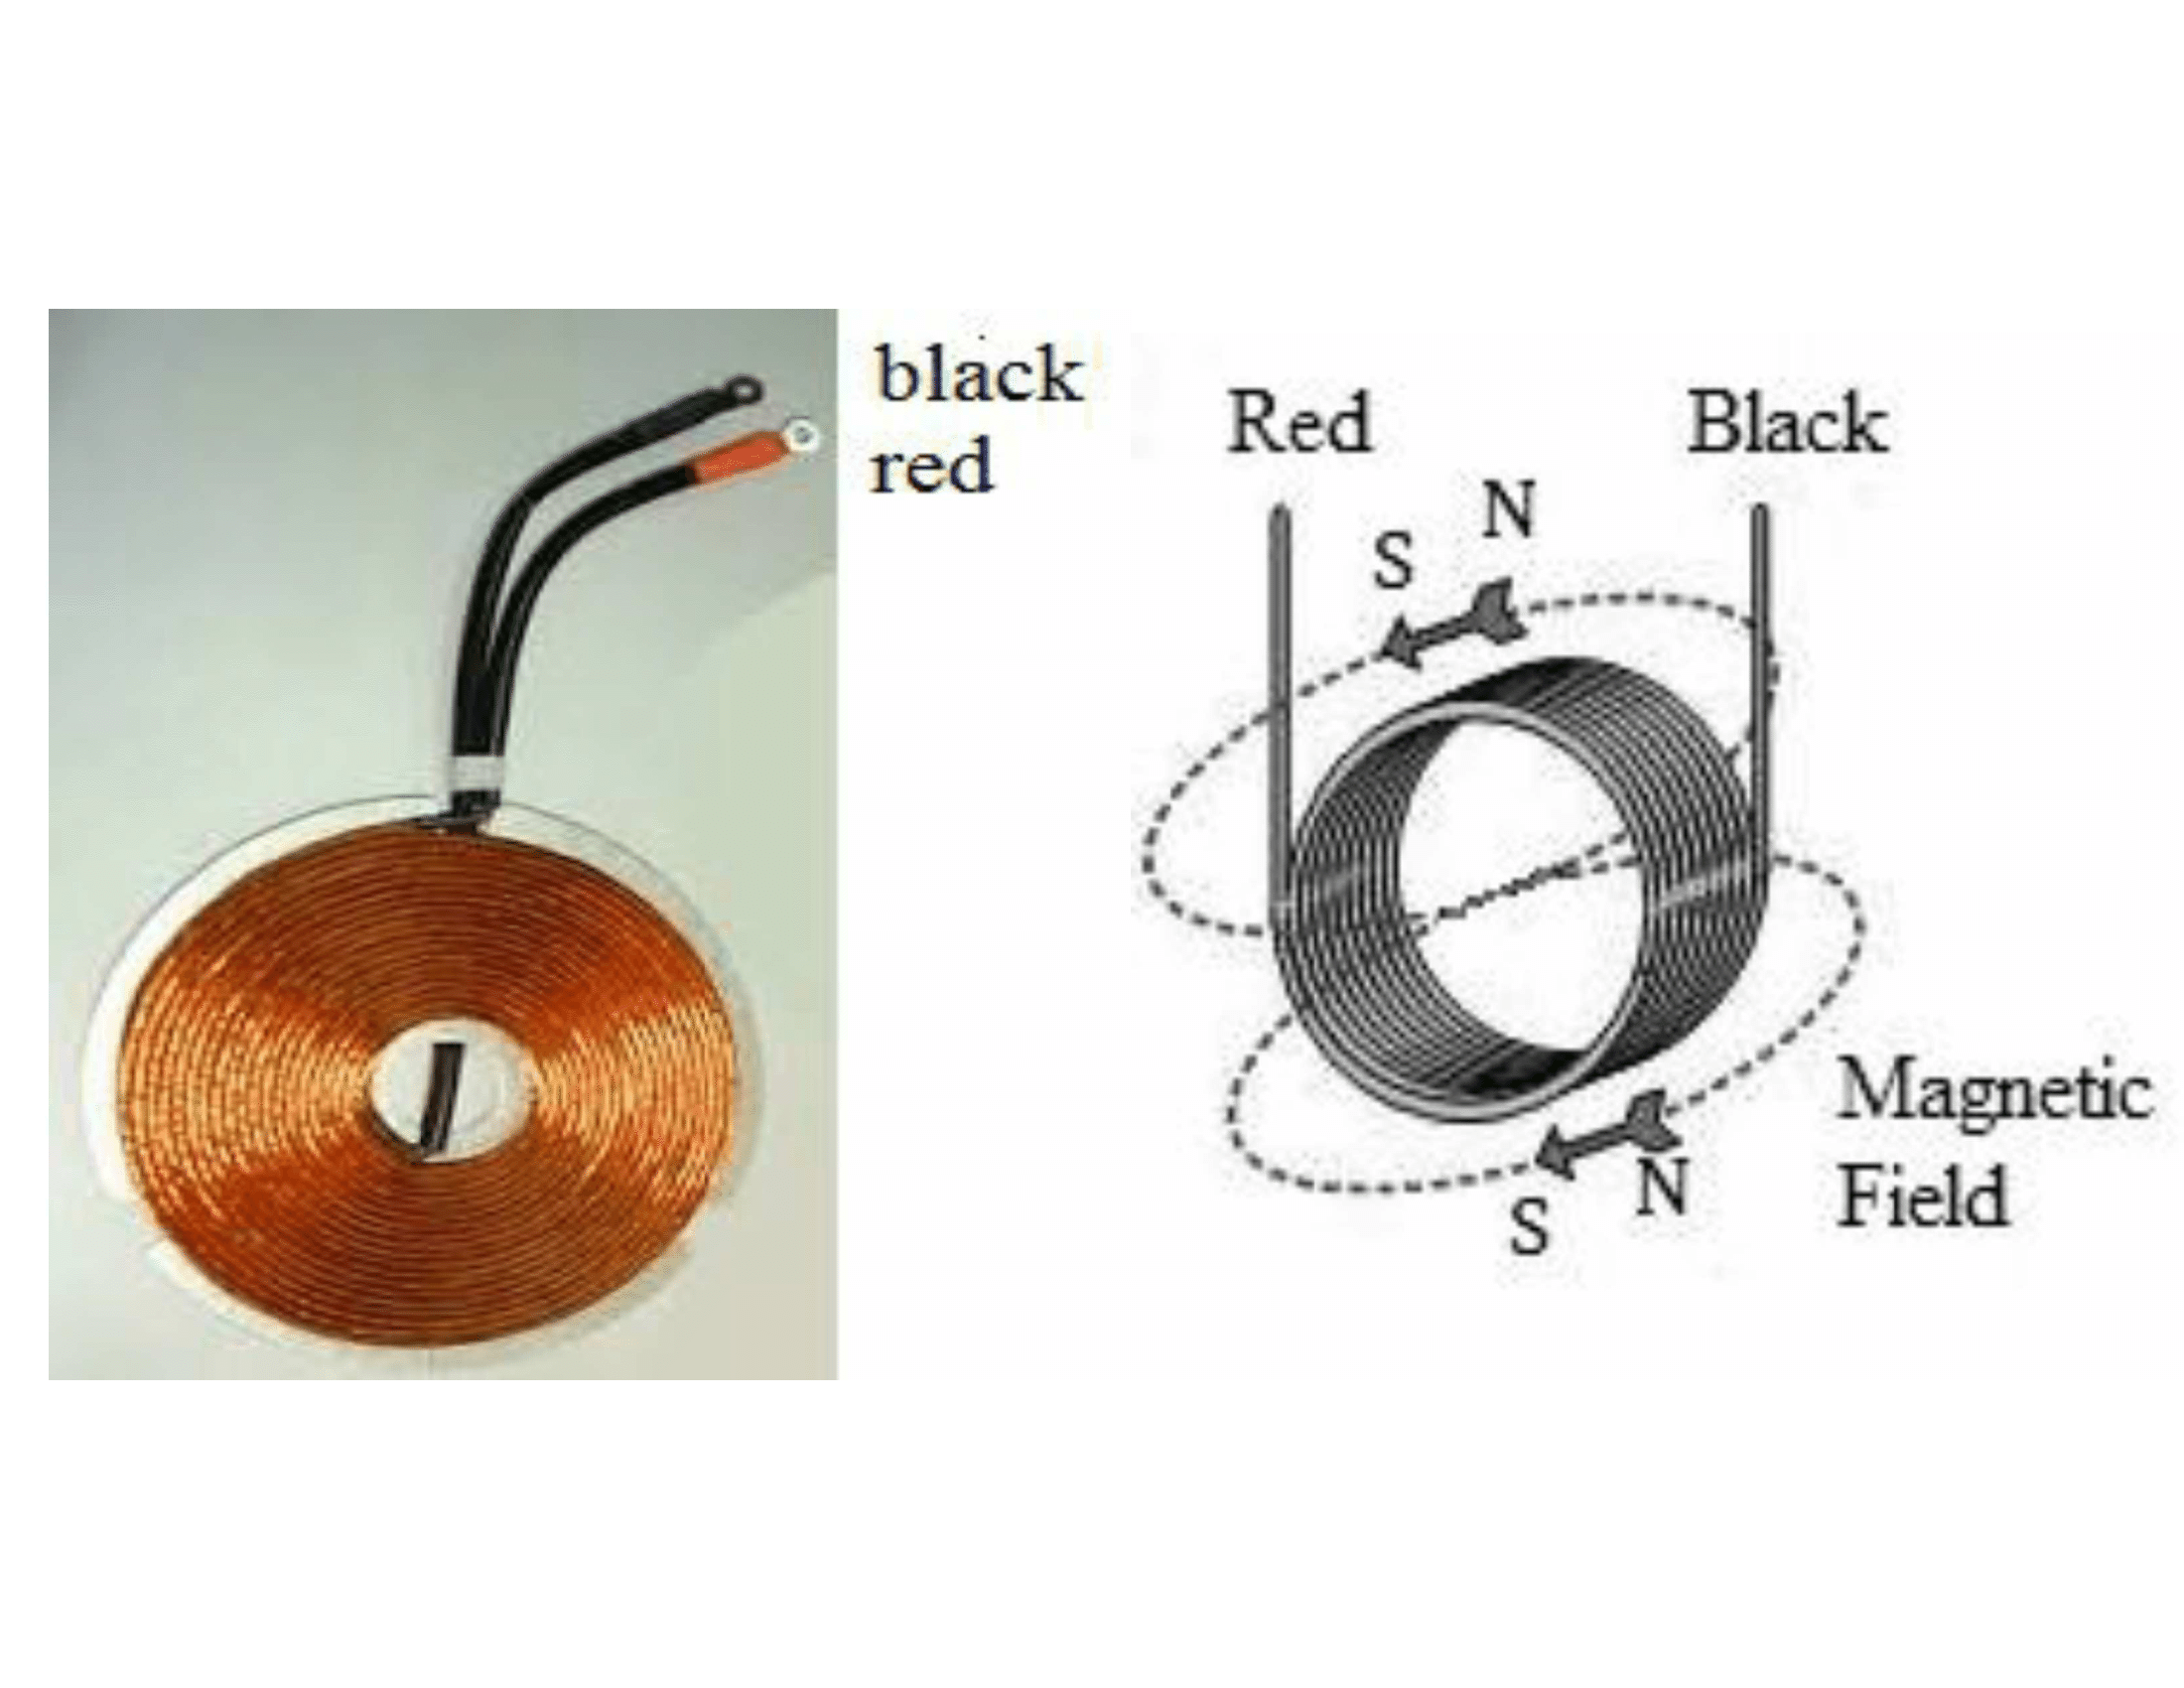
\includegraphics[width=0.8\textwidth]{./Exp4/pic/emf_coil.png}
\caption{Apparatus of the magnetic field sensor}
\label{fig:emfcoil}
\end{figure}

CAUTION: Do not put the magnets very close to a computer! \myskip

\begin{enumerate}
 \item Adjust the height of the stand so that the coil is in the middle of the magnet. Adjust the gap between the magnet poles to about 1 inch so the coil will be close enough to the magnet poles and will be able to pass through the magnet without hitting the pole plates.
 \item Plug the voltage sensor banana plugs into the banana jacks of the induction wand. Connect the voltage sensor to the USB link that is plugged into the computer. Make sure that the voltage sensor cables will not exert any torque on the induction wand as it swings. If you notice this happening, it helps to hold the wires up while recording data. See \ref{fig:voltage_cables}

 \begin{figure}[h]
 \centering
 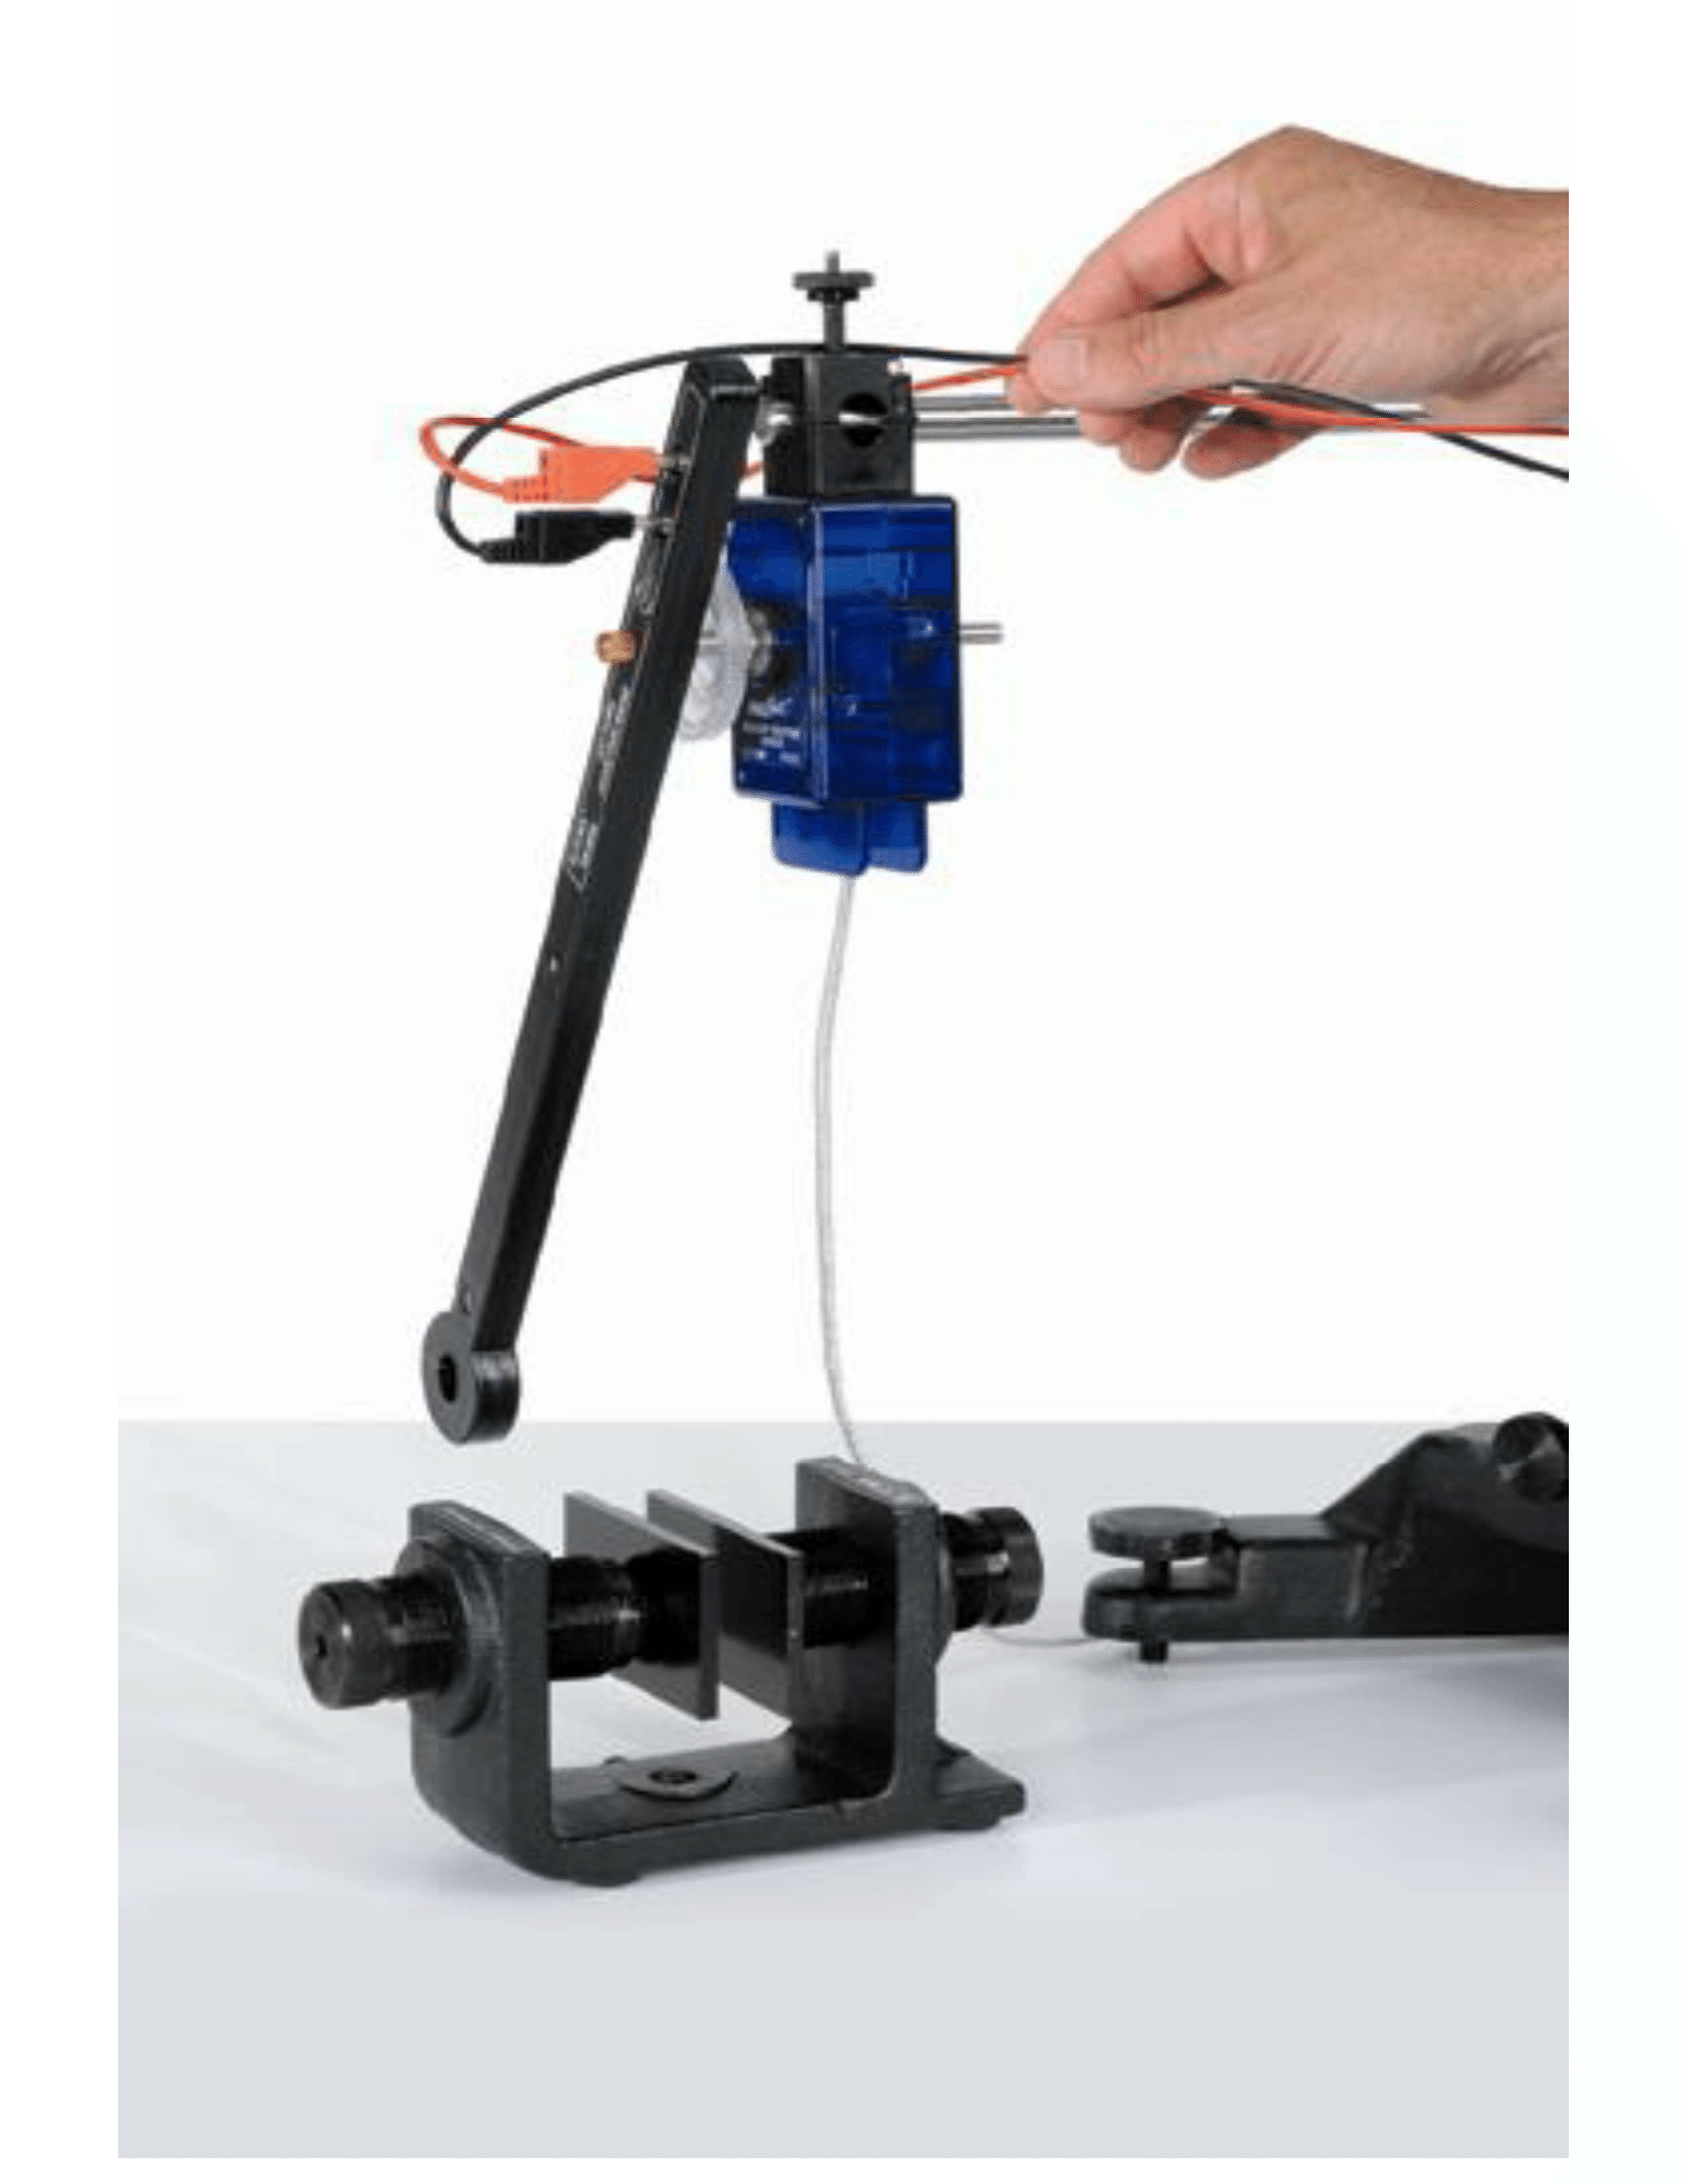
\includegraphics[width=0.4\textwidth]{./Exp4/pic/voltage_cables.png}
 \caption{Voltage sensor cables}
 \label{fig:voltage_cables}
 \end{figure}

 \item Attach the rotary motion sensors USB link to the computer.
 \item Attach the magnetic field sensor to the computer. Notice that the magnetic field sensors probe has two white dots: one for sensing perpendicular magnetic field lines (as shown in Figure \ref{fig:mag_sensor}) and the other for axial field lines. You will use the perpendicular sensing element. Note the direction of the arrow in the figure. Make sure DataStudio is set to measure in units of Tesla to simplify calculations.

 \begin{figure}[h]
 \centering
 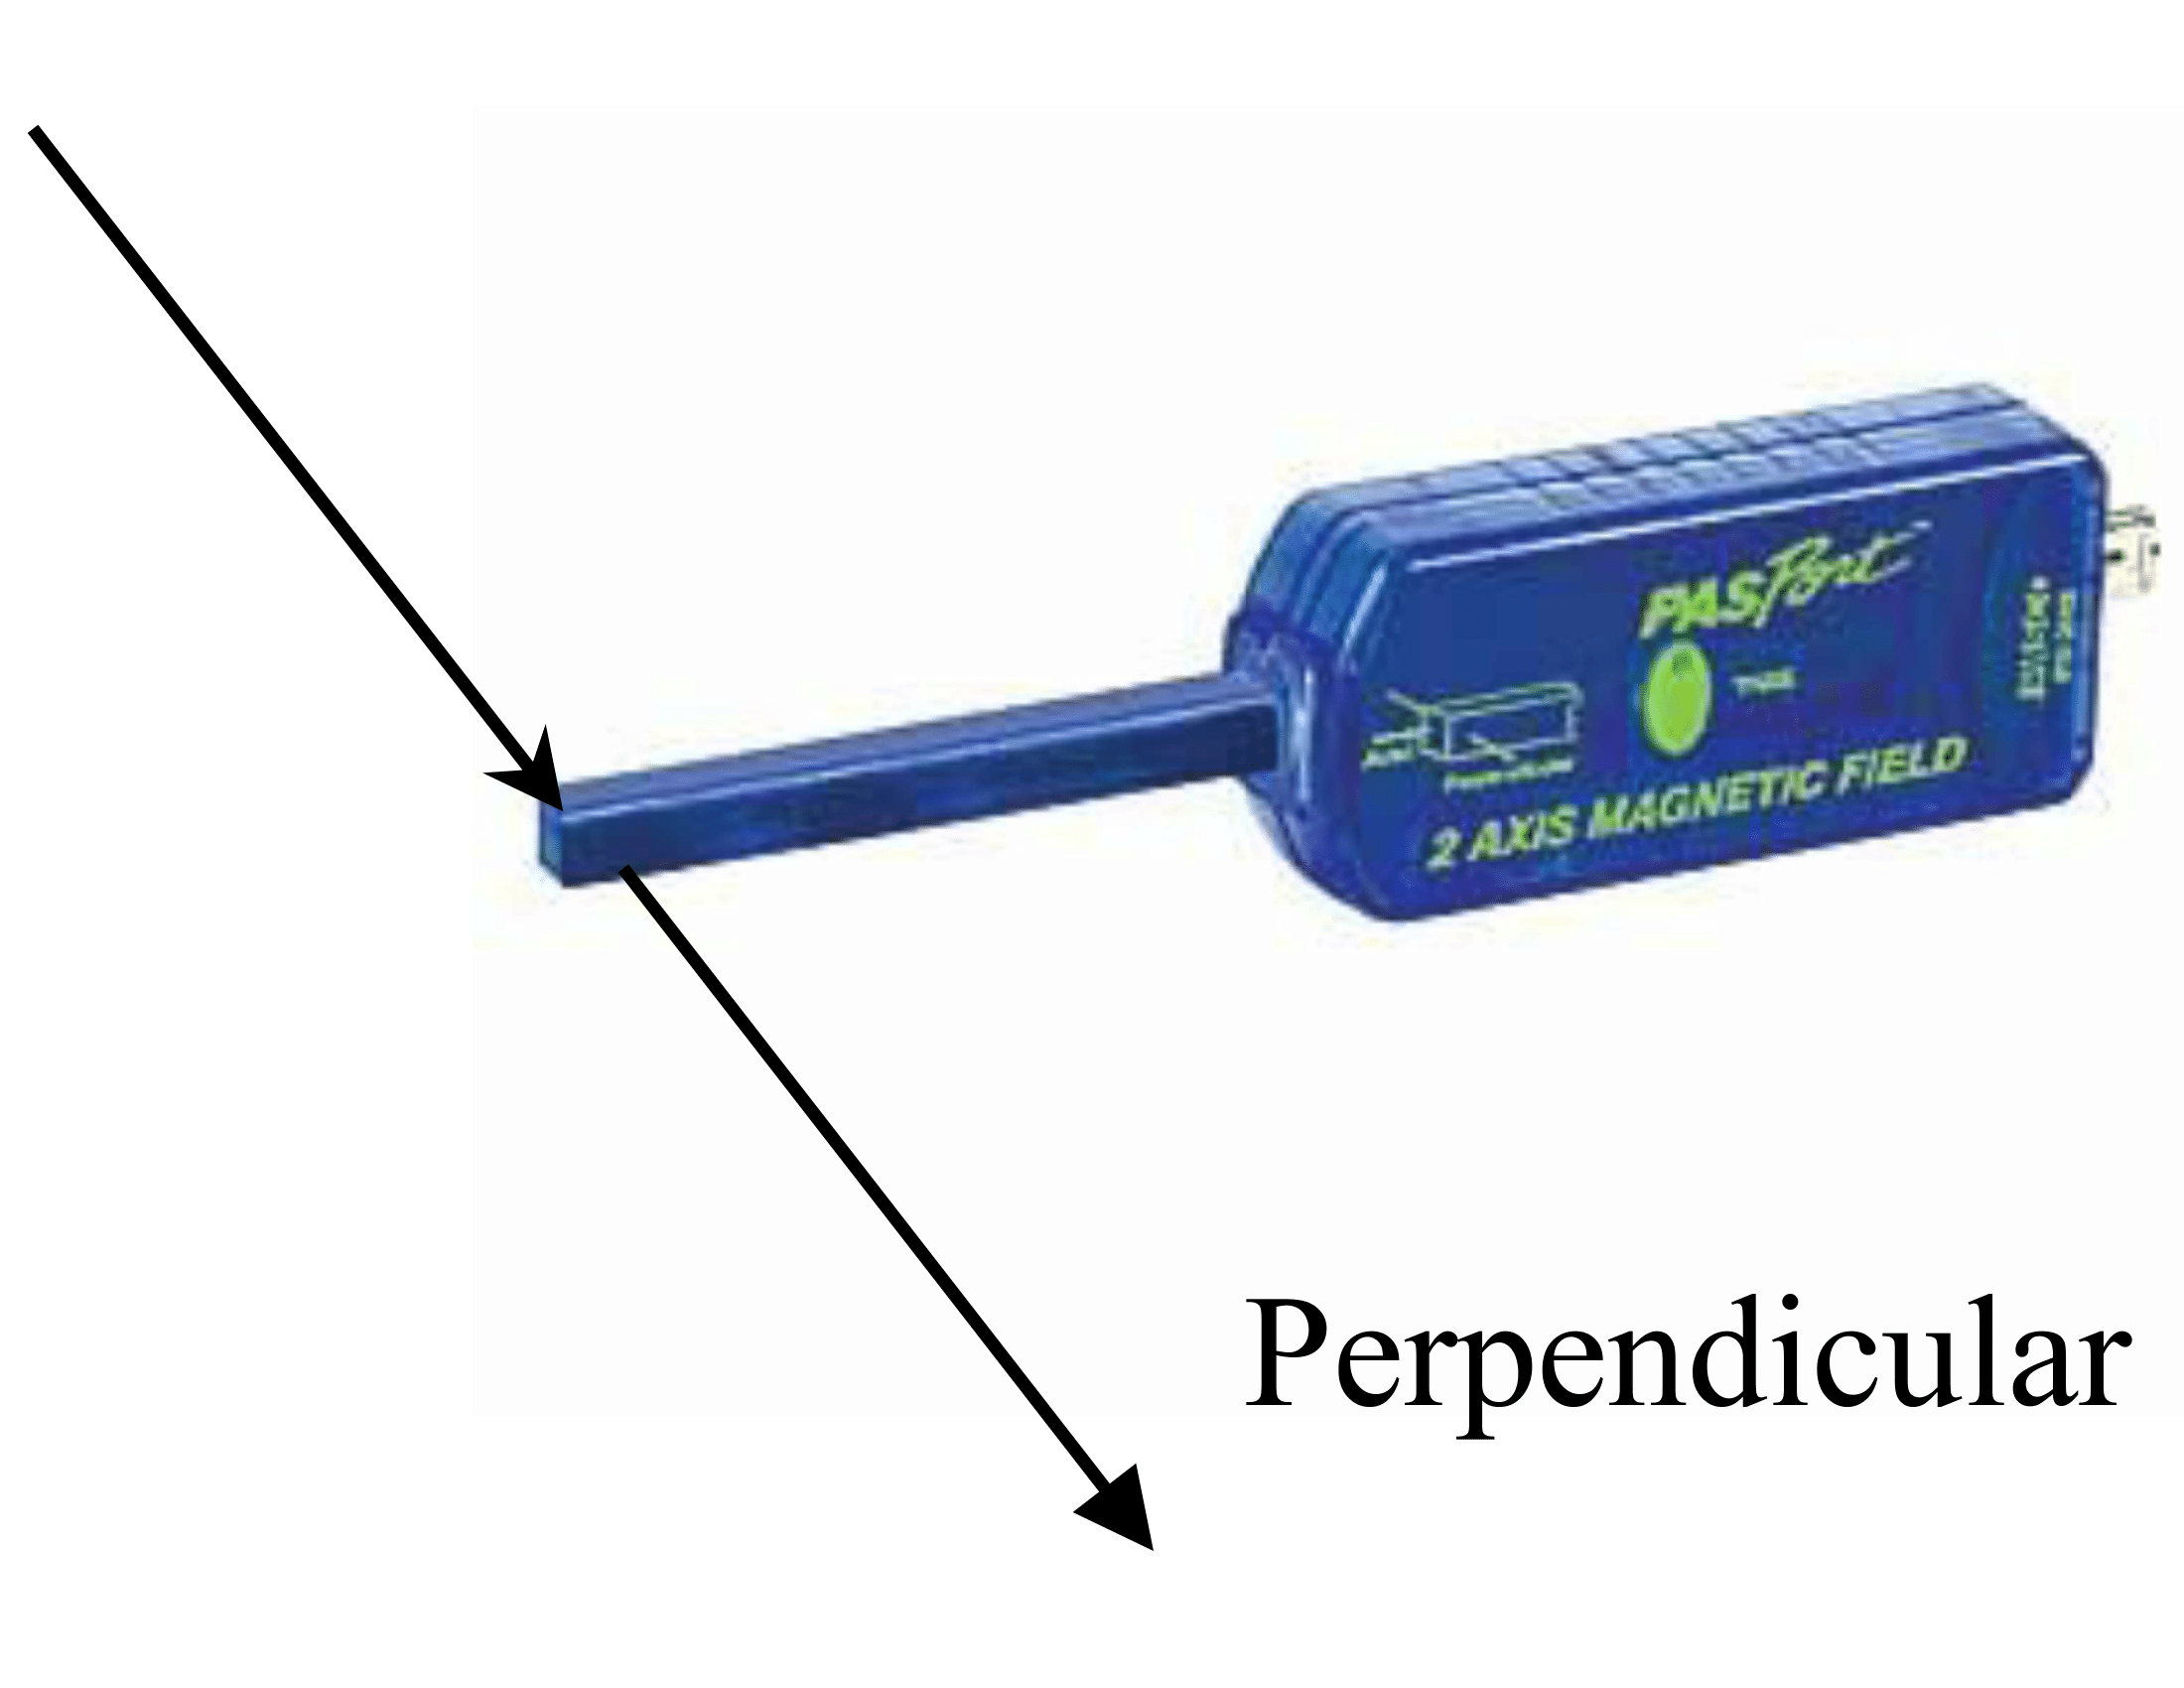
\includegraphics[width=0.5\textwidth]{./Exp4/pic/mag_sensor.png}
 \caption{Magnetic field sensor}
 \label{fig:mag_sensor}
 \end{figure}

 \item Click on ``InducedEMF" on computer desktop. Make sure that the sampling rate setting (which can be found in the Setup menu) shows the following: Magnetic field: 1 Hz, Angle: 10 Hz, Voltage 1000 Hz.

 \item Pull the magnet out of the setup so that you can place the magnetic field sensor in between the pole plates. Hold the magnetic field sensor such that the perpendicular sensing element is in between and near the center of the two magnetic pole plates. See Figure \ref{fig:mag_measure} for reference.

 \begin{figure}[h]
 \centering
 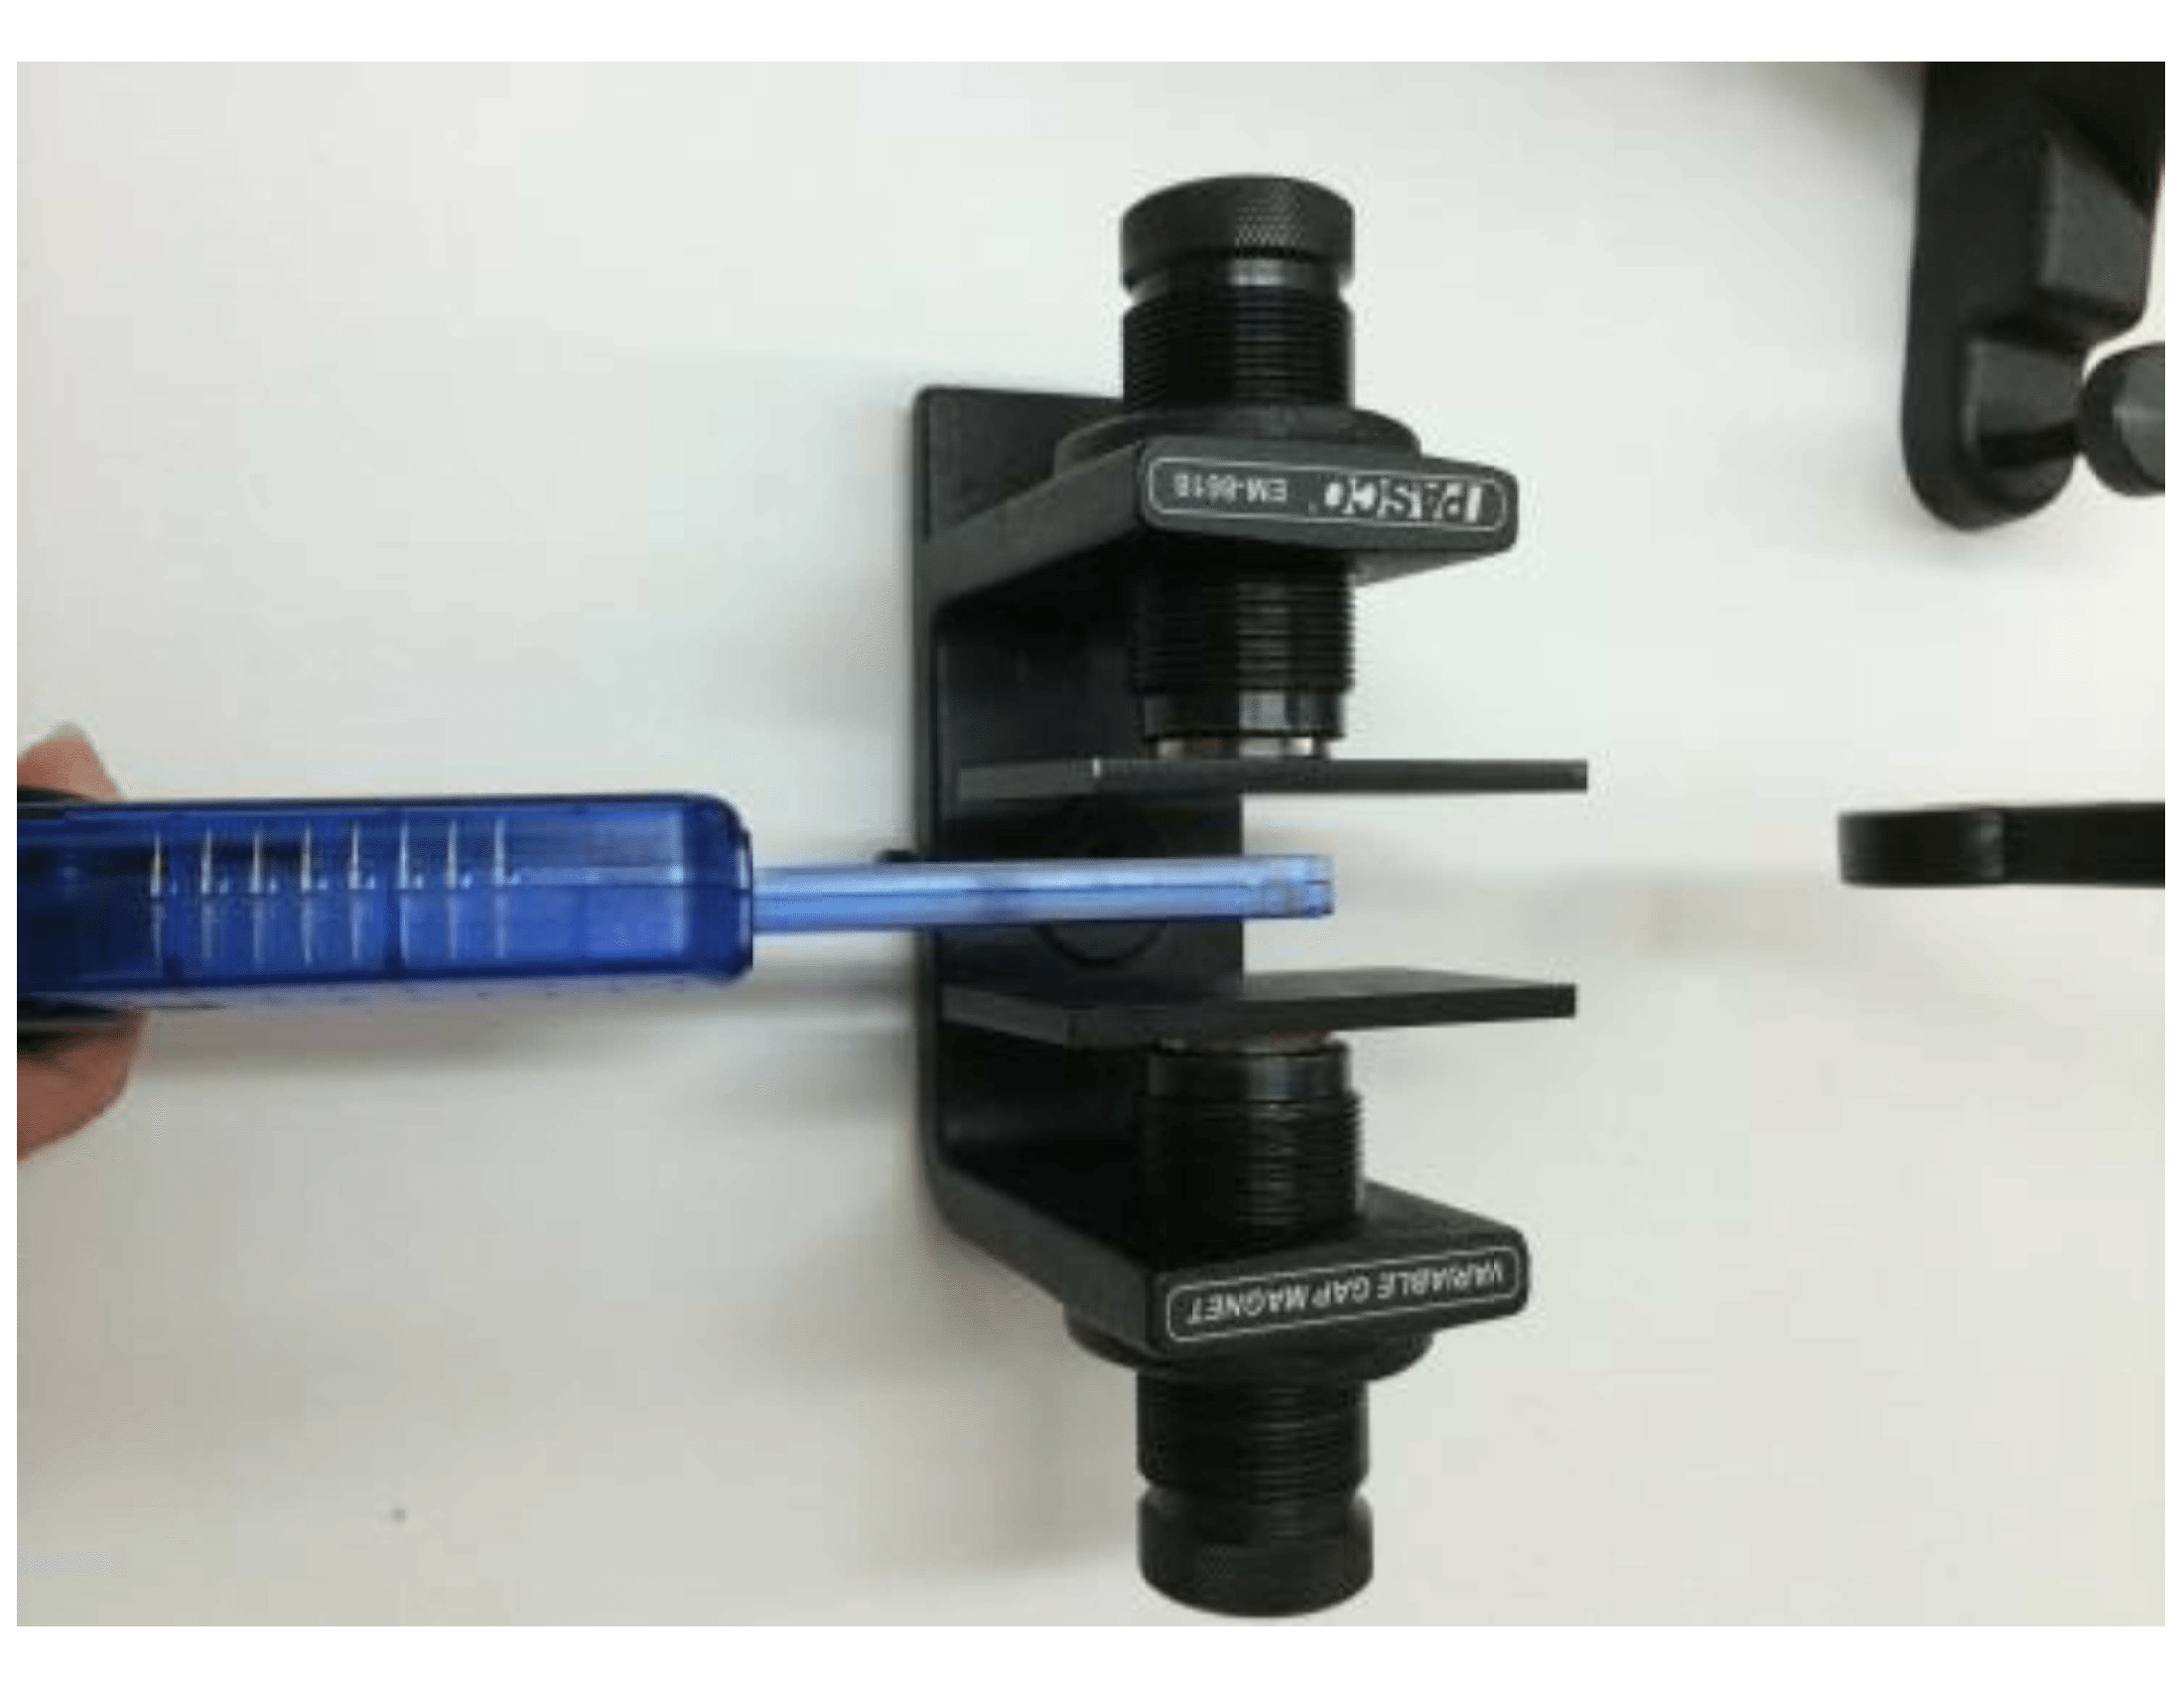
\includegraphics[width=0.5\textwidth]{./Exp4/pic/mag_measure.png}
 \caption{Magnetic field sensor}
 \label{fig:mag_measure}
 \end{figure}

 \item Click Start to measure the maximum magnetic field strength between the poles. Hold the sensor in the center for around 6 seconds. Click Stop. You will see a straight line in the magnetic field pane. Record the mean value of the measured magnetic field. From the sign of the recorded value determine the direction of the magnetic field between the pole plates. Note which pole of the magnet is the north pole.

 \item Move the sensor 1 cm away from the center of the pole plates and repeat the measurement of the magnetic field at this new spot. Now move it 2 cm away from the center. What do you notice? How might this contribute to uncertainty in the experiment.

 \item Put the magnet back in the setup as shown in Figure \ref{fig:emfsetup}. Again, make sure that the coil can pass through the gap without hitting pole plates. Pull the wand back and click Start. Release the wand, allowing it to swing through the magnet once and then click Stop.

 \item Use the Magnifier tool to enlarge the portion of the Voltage vs. Time graph where the coil passed through the magnet.

 \item Click and drag the mouse over the first peak to highlight the first peak and find the average voltage by getting the mean of the highlighted part of the graph. Try to select the same amount of data points on each side of the peak.

 \item Use the Smart Tool to determine the difference in time (t) from the beginning to the end (the width) of the first peak.

 \item Calculate the value of the average EMF using Equation (\ref{eq:emf}) and the B field you got from the previous section. Compare this value to the average voltage value measured from your graph.

 \item Identify on the graph where the coil is entering the magnet and where the coil is leaving the magnet.

 \item Is the EMF of the first peak positive or negative? Does the sign of the EMF correspond to the direction expected using Lenz's Law?

 \item Why is the sign of the EMF of the second peak opposite to the sign of the first peak?

 \item Why is the EMF zero when the coil passes through the exact center of the magnet?

\end{enumerate}
